\chapter{State of the art}
\label{chap:sota}


\localtableofcontents


\section{Introduction}
% region: intro
The development of neural networks and their performance has been accompanied by
a significant increase in their size and more particularly in the number of
weights of which they are composed. In parallel, the development of these
networks has given rise to various applications, particularly embedded ones,
whose resources are highly constrained in terms of computing power, energy
consumption or memory footprint. In conjunction with the increase in the size of
these networks, compression methods have been developed, in order to enable the
use of these networks in the said applications. his chapter focuses on these
latter techniques and presents state-of-the-art neural network compression
methods, mostly based on reducing the number of weights. First, we will explore
ad-hoc architectures, referred to here as "Efficient Architectures". These
networks are lightweight networks that revolve around a core technique to reduce
their size while preserving performance as much as possible. Subsequently, we
will discuss \ac{NAS}, a method that automates the discovery of optimal network
architectures tailored to specific tasks or constraints, potentially leading to
more compact and efficient designs. Following this, we will examine fast
convolution techniques, which aim to accelerate the computation of convolutions
in neural networks, thereby reducing both the runtime and computational
resources required. Next, we will delve into \ac{KD}, a process by which the
knowledge of a larger, more complex network (denoted the \emph{teacher}) is
transferred to a smaller, more efficient network (denoted the \emph{student}),
enabling the latter to achieve comparable performance with a reduced footprint.
Afterwards, we will address weight operations techniques, including methods such
as low-rank factorisation and other linear algebra techniques, which help to
reduce the complexity and size of the networks by exploiting inherent
redundancies and structures in the weight matrices. Lastly, we will consider
Neural Network Pruning, a set of techniques that involve the removal of
redundant or insignificant connections and weights from the network, resulting
in a sparser and more computationally efficient model.\\

% endregion: intro

\section{Efficient Architectures}

% region: depthwise separable convolutions

One of the early approaches to achieving efficiency in neural network
architectures is the use of depthwise separable convolutions. This technique,
employed in \cite{howard2017mobilenets} and \cite{DBLP:conf/icml/TanL19},
separates the standard convolution operation into two separate steps: a
depthwise convolution and a pointwise convolution (see
\cref{fig:sota:depthwise_conv_vs_standard_conv}). By decomposing the operations
in this manner, the computational complexity is significantly reduced while
still retaining the ability to capture spatial and channel-wise information.
Consider a $C_\text{in}$-channels input feature map of arbitrary width and
height and $C_\text{out}$ convolution kernels of size $k\times k \times
C_\text{in}$. A standard convolution algorithm will need $C_\text{in} \times
C_\text{out} \times k \times k$ \ac{MAC} operations to produce a $1 \times 1
\times C_\text{out}$ element of the output feature map. In contrast, a depthwise
separable convolution algorithm will first apply a $k\times k \times 1$
convolution kernel to the $C_\text{in}$ channels and then perform $C_\text{out}$
pointwise convolutions with $1\times 1 \times C_\text{in}$ kernels to produce
the same $1\times 1 \times C_\text{out}$ element. This reduces the number of parameters to
$C_\text{in} \times (C_\text{out} + k \times k)$, essentially reducing the
number of computations needed to produce a $1 \times 1 \times C_\text{out}$
element by a factor of\\

$$\displaystyle\frac{C_\text{out}\times k \times k}{C_\text{out} + k \times k}.$$\\

\begin{figure}[htbp]
\centering
\subfloat[Standard Convolution\label{fig:sota:standard_convolution}]{
    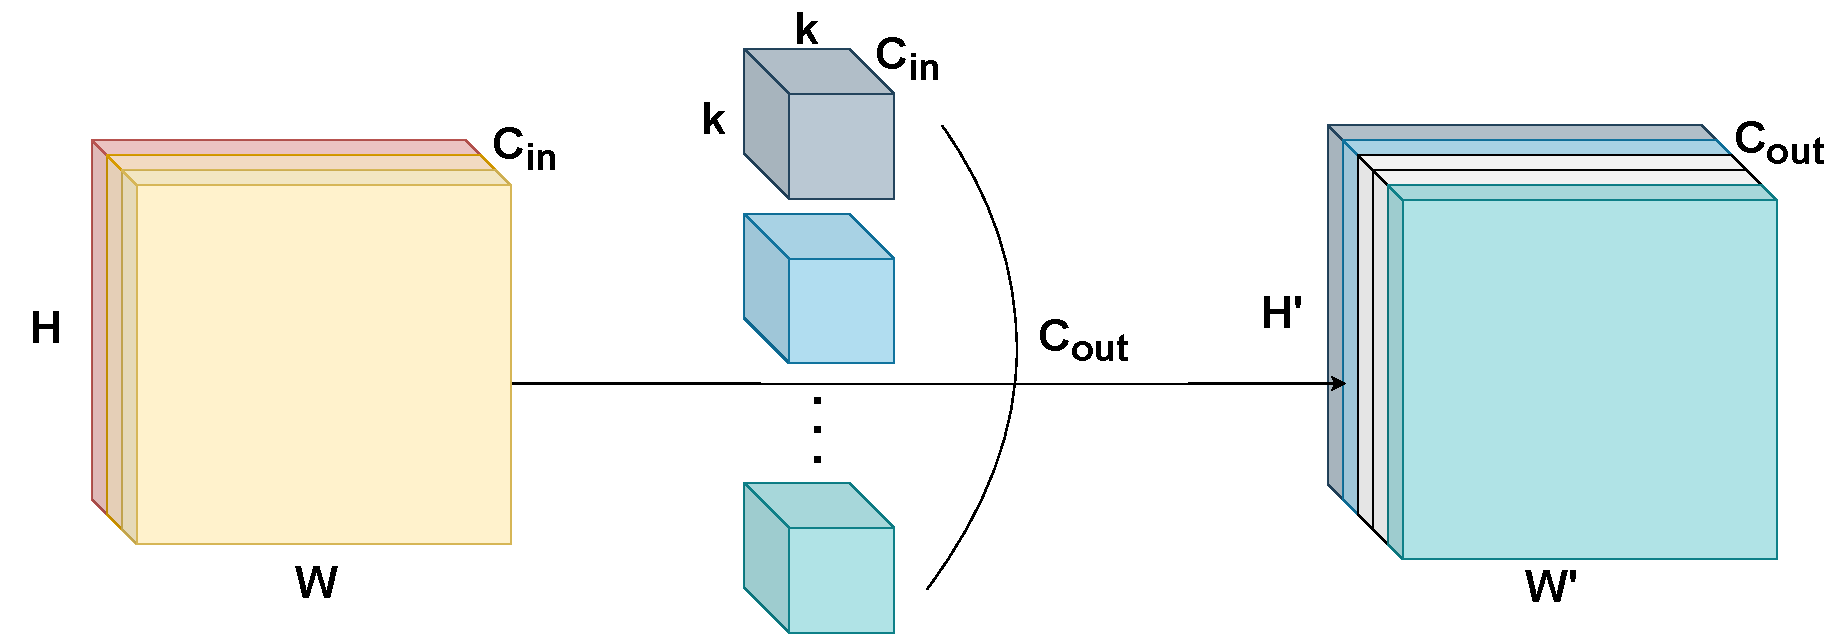
\includegraphics[width=0.70\textwidth]{chapter_sota/assets/standard_conv_scheme.pdf}}\\
    \vspace{1cm}
\subfloat[Depthwise Separable
    Convolution\label{fig:sota:depthwise_convolution}]{
    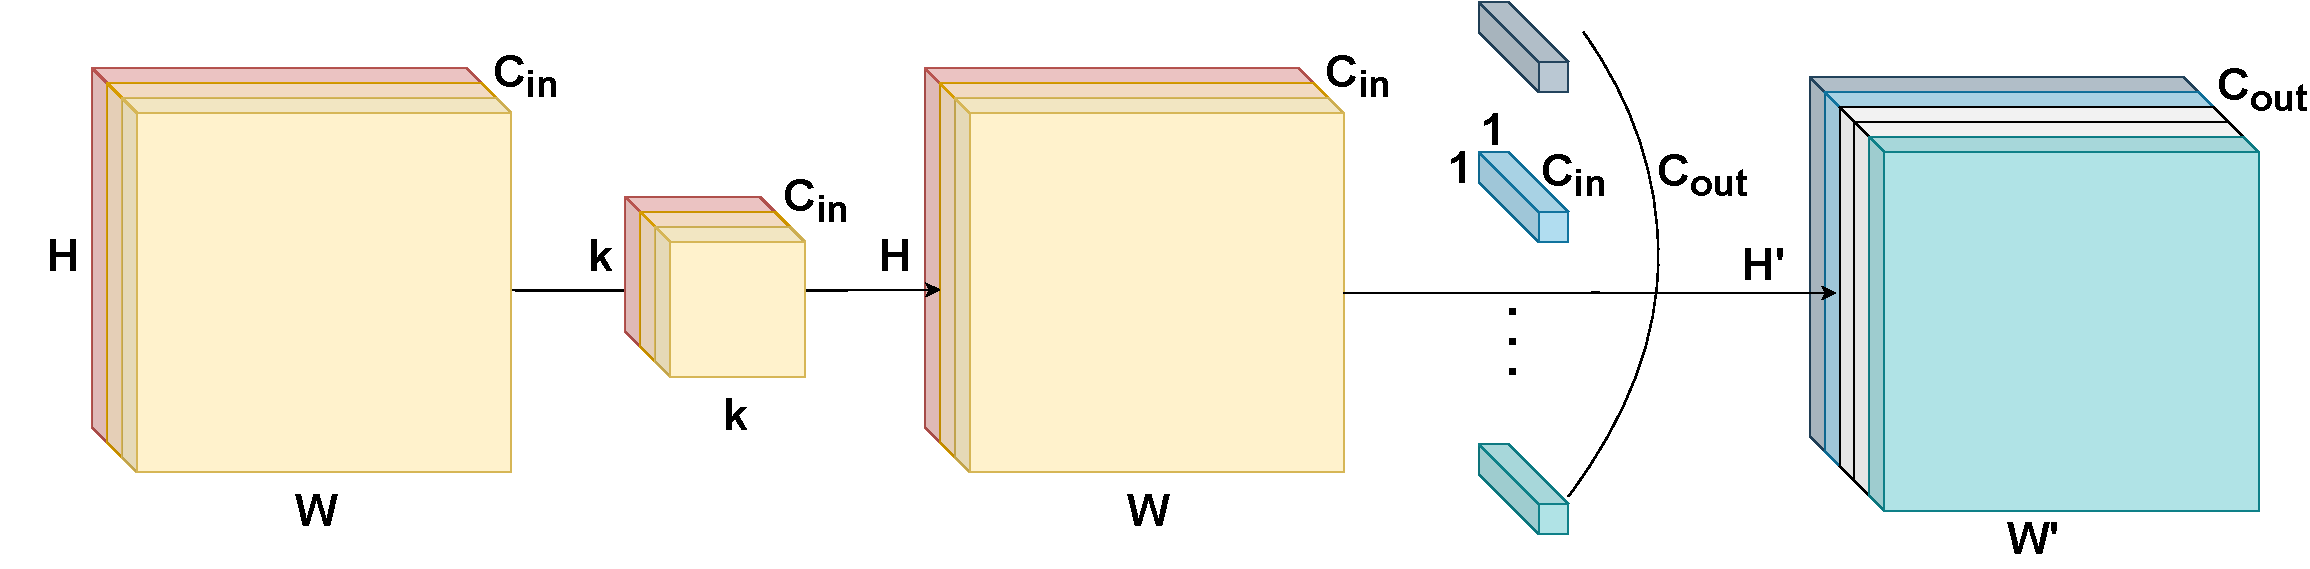
\includegraphics[width=0.70\textwidth]{chapter_sota/assets/depthwise_sep_conv_scheme.pdf}}
    \caption{Illustration schemes of the standard and depthwise separable
    convolution. The standard convolution uses $C_\text{out}$ kernels of size
    $k\times k \times C_\text{int}$. The depthwise separable convolution is
    split into two steps: \emph{(i)}   a convolution with $C_\text{in}$ kernels
    of size $k \times k$ and \emph{(ii)} a convolution with $C_\text{out}$
    kernels of size $1\times 1 \times C_\text{int}$.
    Best viewed in colours.}
\label{fig:sota:depthwise_conv_vs_standard_conv}
\end{figure}

% endregion: depthwise separable convolutions

% region: fire module
An alternative approach for designing efficient architectures involves the
integration of \emph{fire modules}, as proposed in
\cite{DBLP:journals/corr/IandolaMAHDK16}. These modules aim to minimise
computational requirements by employing two distinct strategies: \emph{(i)}
diminishing the number of input channels supplied to the following conventional
$k\times k$ convolutions and \emph{(ii)} substituting a portion of the
resource-intensive $k\times k$ convolutions with pointwise convolutions, which
possess $k^2$ times fewer parameters. The initial strategy is applied within the
\emph{Squeeze Layer}, which serves to decrease the number of input channels
delivered to the \emph{Expand Layer}, subsequently reducing the parameter count
in the \emph{Expand Layer} kernels. The second strategy is implemented in the
\emph{Expand Layer}, where some $3\times3$ convolutions are replaced with
$1\times1$ variants. Although the $1\times1$ convolutions capture less spatial
information, they are significantly less computationally demanding.\\

\begin{figure}[htbp]
    \centering
    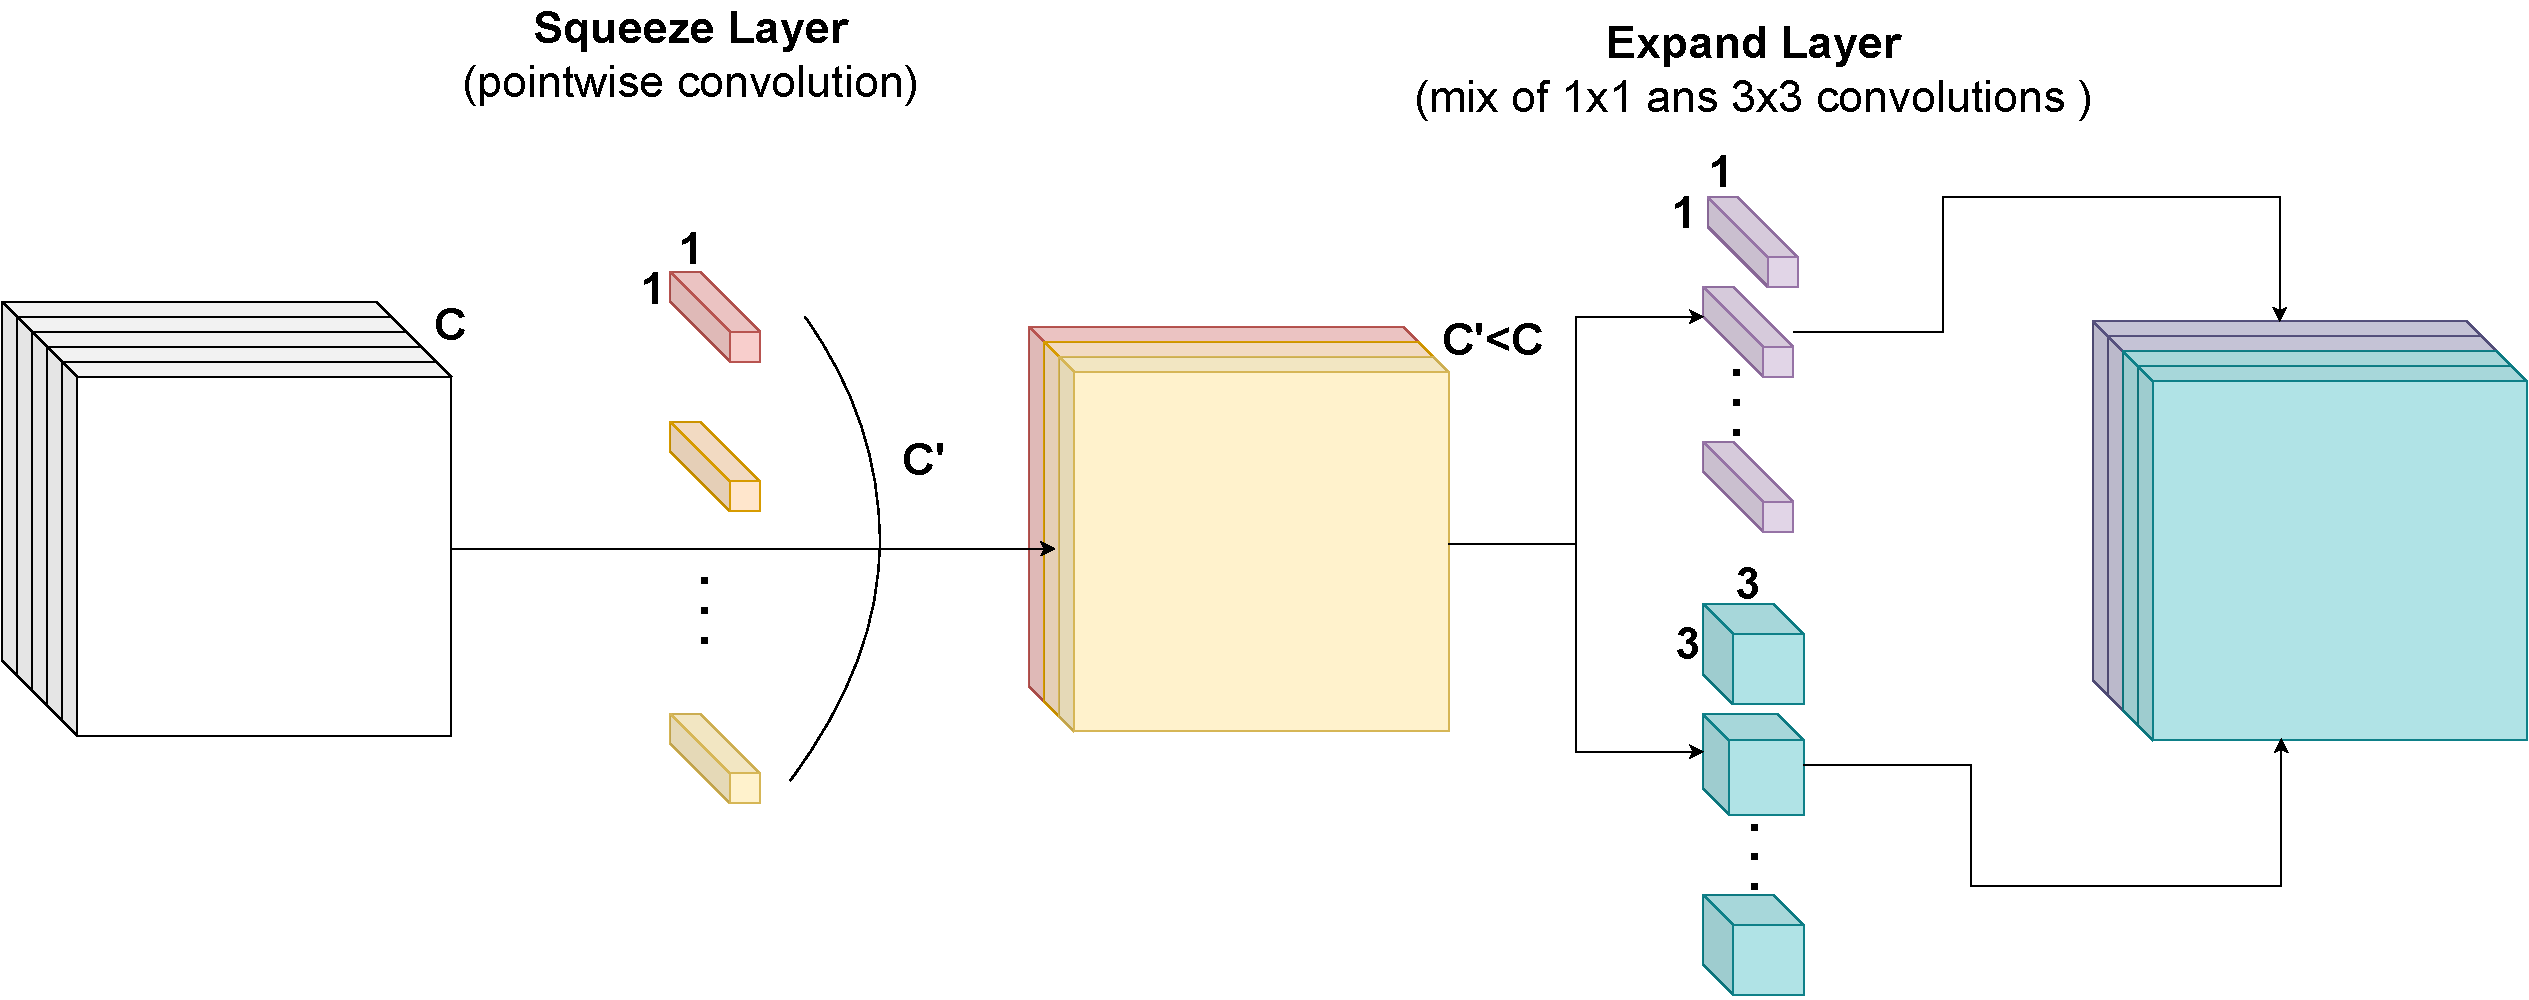
\includegraphics[width=0.70\textwidth]{chapter_sota/assets/fire_module.pdf}
    \caption{Illustration scheme of the fire module. The fire module is composed
    is composed of a \emph{squeeze layer} (pointwise convolution designed to
    reduce the number of channels fed to the following layer) and an
    \emph{expand layer} (convolution with mixed $1\times1$ and $3\times3$
    kernels. The $1\times1$ kernels replace some of the $3\times3$ kernels,
    being less computationally intensive.). Best viewed in colours.}
    \label{fig:sota:fire_module}
\end{figure}

% endregion: fire module

% region: shufflenet

Pushing further the concept of depthwises separable convolutions,
\cite{ZhangShuffleNet} introduces pointwise group convolutions and channel
shuffle operations to enhance efficiency while maintaining accuracy. Pointwise
group convolutions were initially introduced in
\cite{DBLP:conf/nips/KrizhevskySH12}, although their original purpose was not
for compression. Instead, group convolutions in
\cite{DBLP:conf/nips/KrizhevskySH12} were used to enable distributed training
across multiple \acp{GPU} with limited memory. However, ShuffleNet
\cite{ZhangShuffleNet} leverages this concept for network efficiency by dividing
the input channels into groups and performing convolutions on each group
independently. This reduces the number of operations and computational cost
compared to traditional convolutions. To counteract the potential loss of
expressive power caused by the separation of channels into groups, ShuffleNet
incorporates \emph{channel shuffle operations} as shown in \cref{fig:sota:shuffle_net}. This technique allows for
information exchange between groups, effectively maintaining accuracy by
ensuring that different groups can capture diverse features in the input.\\

\begin{figure}[htbp]
    \centering
    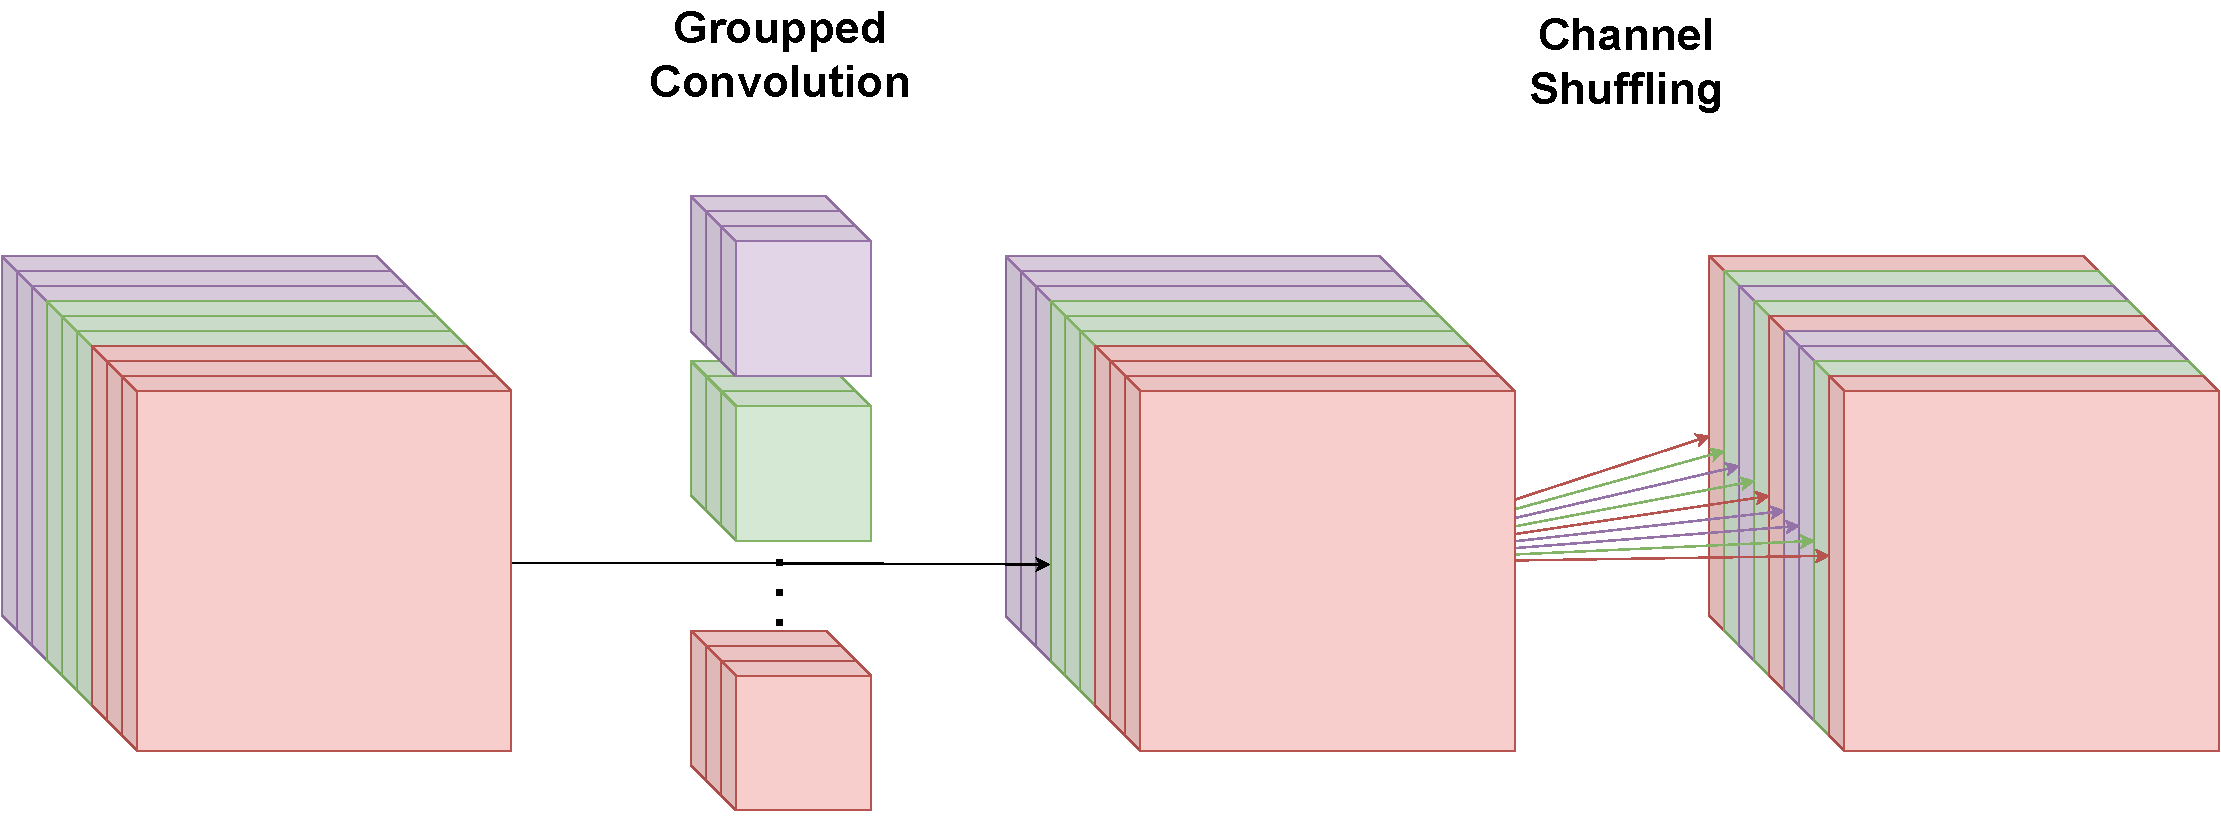
\includegraphics[width=0.70\textwidth]{chapter_sota/assets/group_conv_and_channel_shuffling.pdf}
    \caption{Illustration scheme of groupped convolution with channel shuffling.
    Each filter only acts on a subset of the input tensor (here represented by a
    matching colour). The channels of the yielded tensor are shuffled to ensure
    the subsequent groups can get information all the previous groups. Best
    viewed in colours.}
    \label{fig:sota:shuffle_net}
\end{figure}

Following ShuffleNet, CondenseNet was introduced in
\cite{huang2018condensenet}, incorporating learned group convolutions to further
improve efficiency. Unlike the predefined group convolutions in ShuffleNet,
CondenseNet learns which channels should be grouped together, allowing the
network to adapt its structure for a specific task. This results in better
utilisation of network capacity and reduces redundancy. CondenseNet levrages the
DenseNet architecture \cite{huang2017densely} to further improve performances.
Thanks to the densly connected architecture, features discarded in any layer may
still be recovered in the subsequent ones.\\

\begin{figure}[!h]
    \centering
    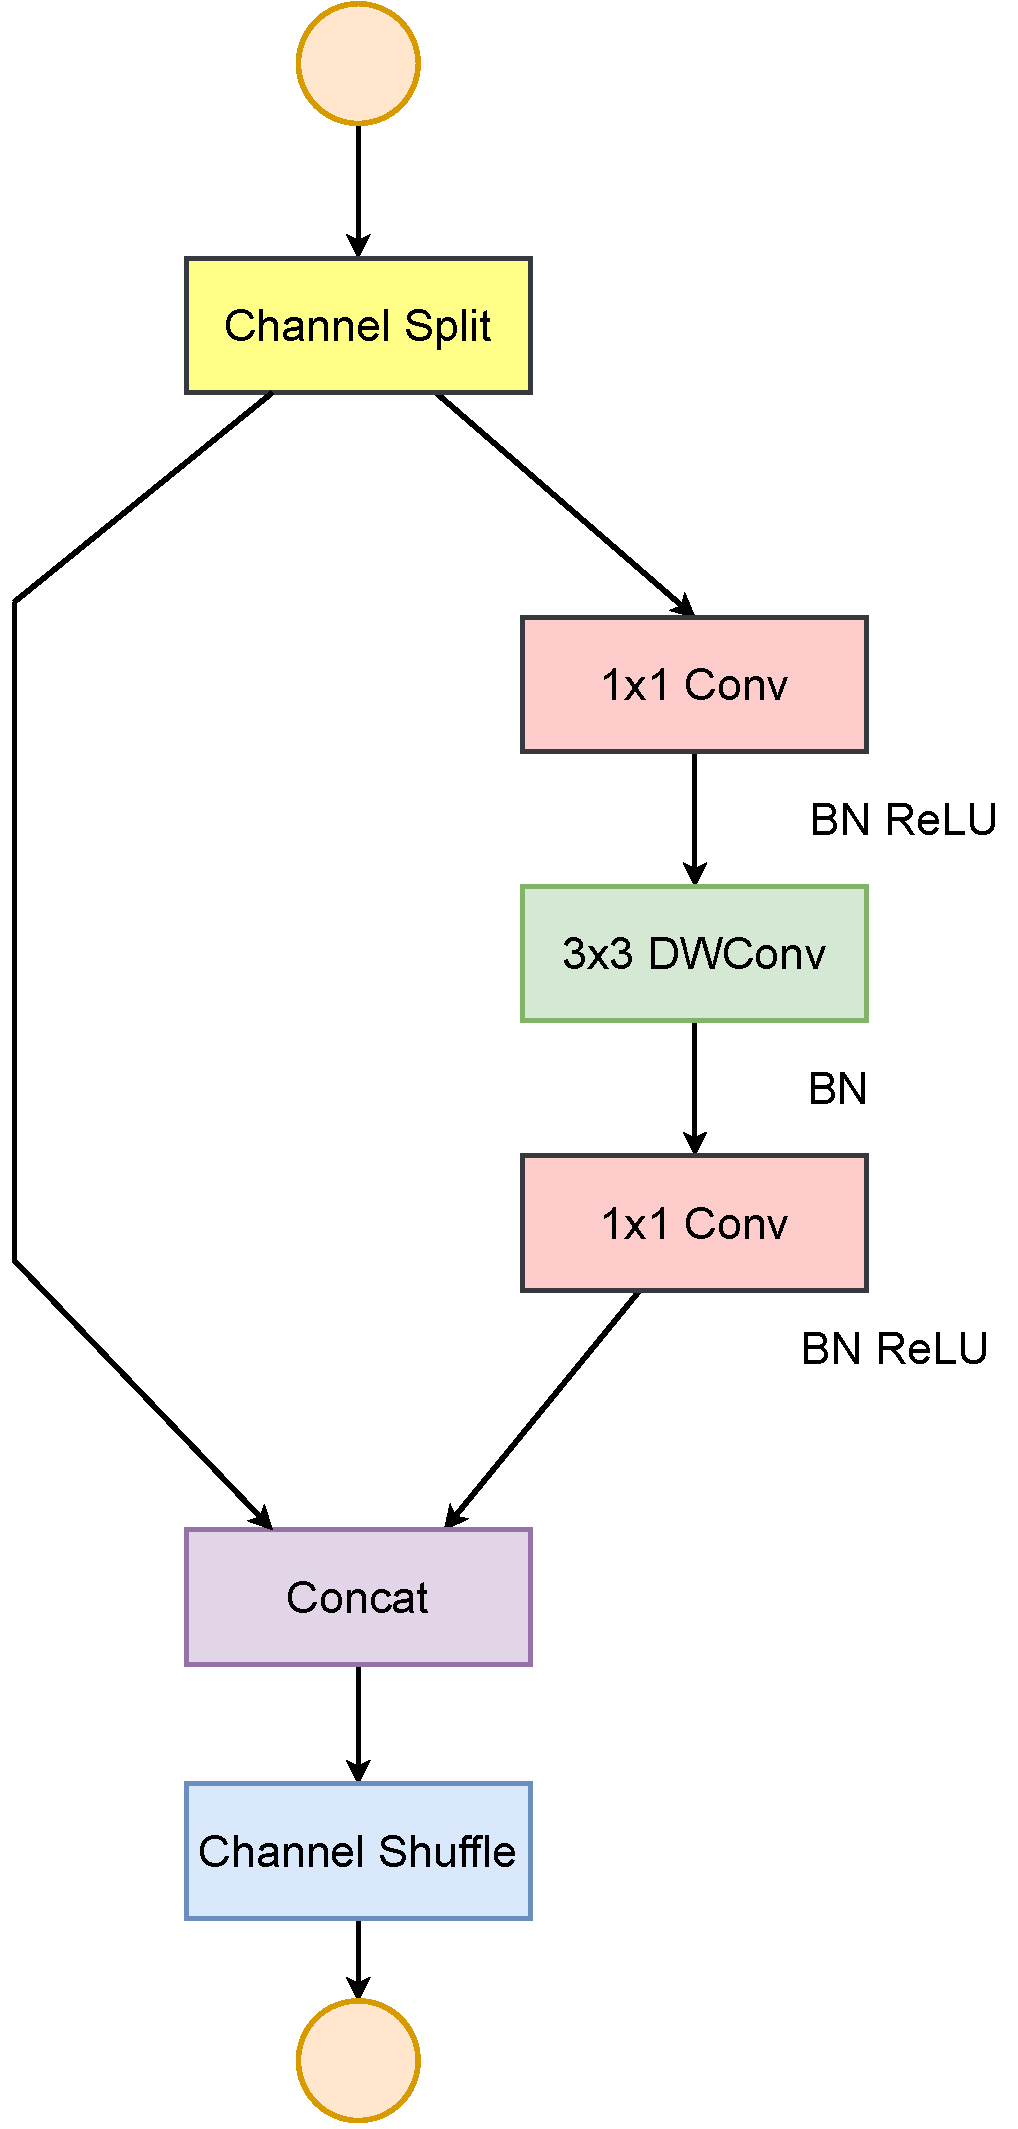
\includegraphics[width=0.3\textwidth]{chapter_sota/assets/channel_split.pdf}
    \caption{Illustration scheme of the path taken by the feature maps after the
    channel split block. Adapted from the original scheme found in \cite{MaShuffleNetV2}}
    \label{fig:sota:channel_split}
\end{figure}

Building on the success of ShuffleNet, ShuffleNetV2 was introduced in
\cite{MaShuffleNetV2} with a focus on improving network efficiency with the
combination of the strided convolution and channel split. Strided convolution
helps reduce the spatial dimensions of feature maps, which in turn reduces the
computation cost. Channel split technique efficiently processes the input
feature maps while maintaining the expressive power of the architecture. Channel
Split works by dividing the input feature maps into two equal parts. One part is
passed through the main branch of the ShuffleNet unit, while the other part goes
through the identity branch, which leaves its input unchanged. In the main
branch, a sequence of pointwise and $3\times 3$ convolutions are performed.
After both the main branch and the identity branch complete their respective
operations, the two parts are concatenated along the channel dimension and the
channels are shuffled. Finally, the output feature maps are passed to the next
ShuffleNet unit in the network. This process is represented in
\cref{fig:sota:channel_split}. This approach balances the computational
efficiency and the expressive capacity of the model.\\
% endregion: shufflenet


Depthwise Separable Convolutions were employed and improved in
\cite{howard2017mobilenets}. \citeauthor{DongMobileNetV2} introduced skip
connections and residual blocks into the MobileNet architecture, initially
proposed in \cite{DBLP:conf/cvpr/HeZRS16}. They also introduced the concept of
inverted residuals and linear bottlenecks. In conventional residual blocks, the
input is first compressed, then expanded, and finally compressed again, after
being added to the original input. With inverted residual bottlenecks, on the
other hand, this process is reversed: the input is first expanded, then a
depthwise separable convolution is applied, and finally, it's compressed again.
In this architecture, the skip connections link the feature maps of smaller
size, instead of the larger ones. This allows for a more memory-efficient
architecture. The standard residual blocks and the inverted residual blocks are
shown in \cref{fig:sota:inverted_vs_residual_blocks}. The linear bottlenecks, on
the other hand, are convolutions without linear activation functions like ReLU.
This takes advantage of the property that high-dimensional feature maps can be
embedded in a lower-dimensional manifold. To do this, it is necessary to use
linear transformations without using an activation function, which could destroy
information.\\

\begin{figure}
    \centering
    \subfloat[Standard Residual Block\label{fig:sota:residual_block}]{%
        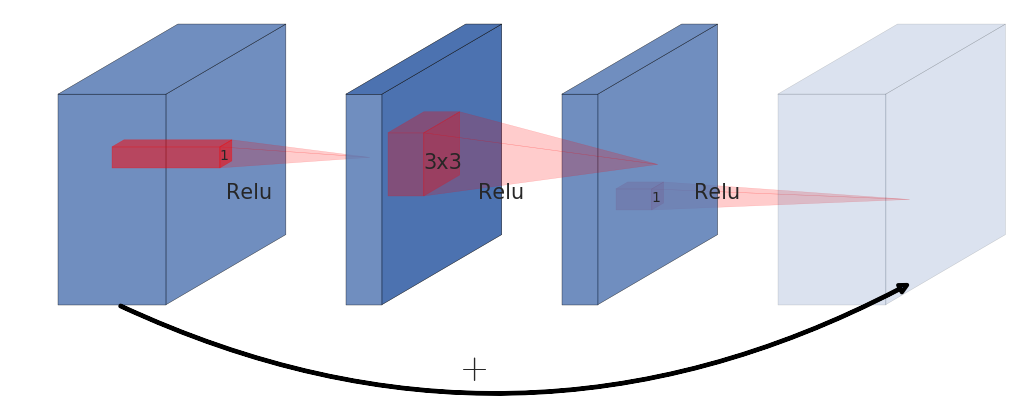
\includegraphics[width=0.49\textwidth]{chapter_sota/assets/mobilenet_v2_residual.png}}
    \subfloat[Inverted Residual Block\label{fig:sota:inverted_residual_block}]{%
        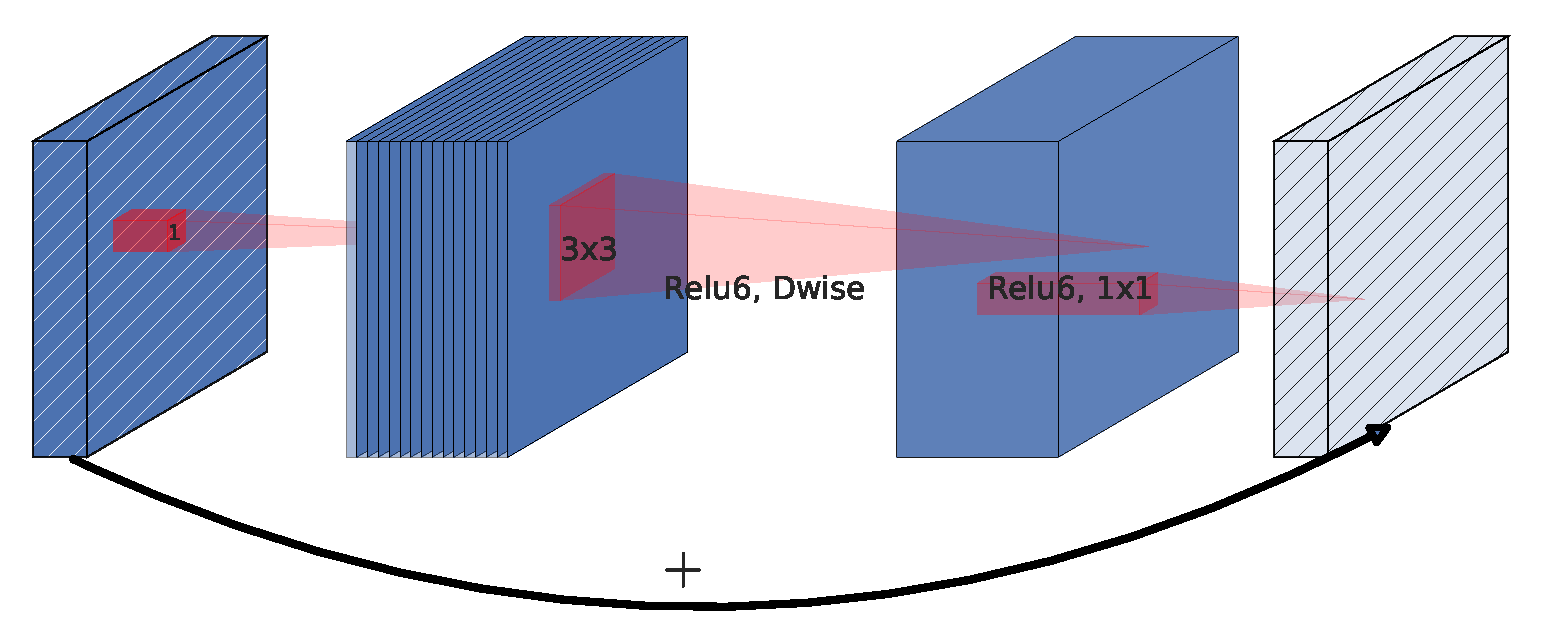
\includegraphics[width=0.49\textwidth]{chapter_sota/assets/mobilenet_v2_inverted_residual.pdf}}
    \caption{Illustration scheme of the residual block and the inverted residual
    block. Note that on the inverted residual block, the feature maps with the lower
    channel count are the ones connected via the skip connection, whereas it is the
    oposite on the standard residual block.Diagonally hatched layers do not use
    non-linearities. The grey color indicates the beginning of the next block. Both
    illustrations are taken from \cite{DongMobileNetV2}. Best viewed in colours.}
    \label{fig:sota:inverted_vs_residual_blocks}
\end{figure}


Advancing from MobileNet and MobileNetV2, its third iteration
\cite{DBLP:conf/iccv/HowardPALSCWCTC19} incorporated \ac{SE} modules initially
introduced in \cite{DBLP:conf/cvpr/HuSS18}. These modules adaptively recalibrate
channel-wise feature responses, amplifying important features and suppressing
less relevant ones. The \ac{SE} module (represented in
\cref{fig:sota:se_module}) performs \emph{squeeze} and \emph{excitation}
operations. The squeeze operation uses global average pooling to create a
channel descriptor that summarises the spatial information for each channel. The
excitation operation uses this descriptor to learn non-linear interactions
between channels through two fully connected layers. The output of this
mini-network are per-channel modulation weights that recalibrate the original
feature maps, scaling or "exciting" them by these weights.\\

The architectures we have just reviewed hinge around specific key techniques
like depthwise separable convolutions, fire modules, channel shuffling, and
\ac{SE} modules, among others. These architectures, while
highly efficient, are manually crafted and necessitate a significant degree of
human expertise, intuition, and time to develop, optimise, and fine-tune. The
manual design of these architectures often relies on a deep understanding of the
tasks at hand, the data they will process, and the constraints of the
environment in which they will operate.However, the process of designing these efficient architectures can be
automated, which is the subject of the next section.\\


\begin{figure}[htbp]
    \centering
    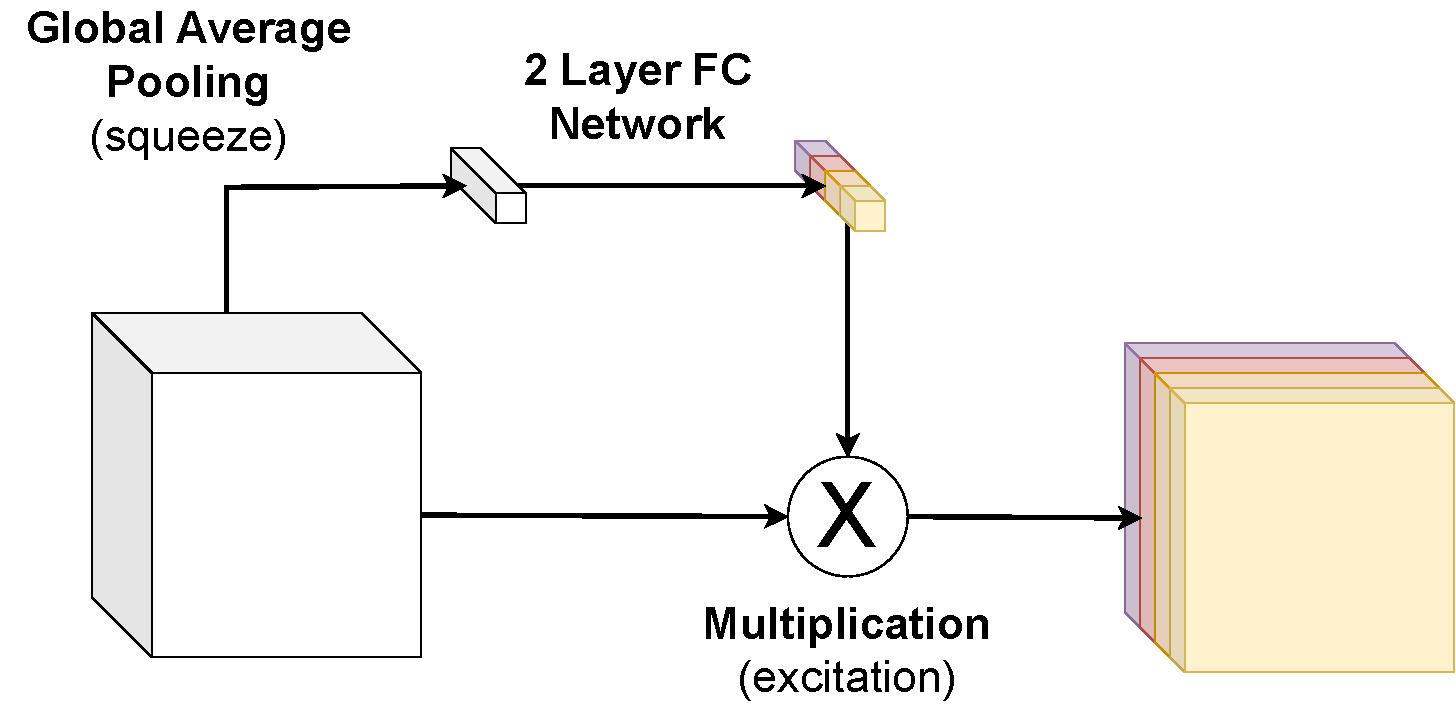
\includegraphics[width=0.70\textwidth]{chapter_sota/assets/SE_module.pdf}
    \caption{Illustration scheme of the \acf{SE} module. The original feature
    map is \emph{squeezed} into a channel descriptor through global average
    pooling. This descriptor is then used to learn the interdependencies between
    the channel through two fully connected layers. The output is then
    multiplied layerwise with the original feature map (\emph{excitation}). Best
    viewed in colours.}
    \label{fig:sota:se_module}
\end{figure}

% Neural Architecture Search
% (NAS). NAS is a method that automates the discovery of neural network
% architectures, potentially leading to more compact, efficient designs and
% reducing the need for manual intervention. Even though NAS might not explicitly
% aim at producing lightweight architectures, it can still yield designs that
% strike a good balance between performance and computational cost. By using
% automated methods to search for optimal architectures, it is possible to further
% enhance the efficiency of neural networks, opening up new possibilities for
% their deployment in resource-constrained environments. This represents an
% exciting area of ongoing research and development in the field of neural
% networks.